\documentclass[twoside,11pt]{article}

\usepackage{aa228-jmlr2e}
\usepackage{lipsum}
\usepackage{listings}
\usepackage{graphicx}
\usepackage{booktabs}
\graphicspath{{"./results/"}}

\usepackage[utf8]{inputenc}
\usepackage{textcomp}
\DeclareUnicodeCharacter{00B1}{\ifmmode\pm\else\textpm\fi}
\usepackage{listingsutf8}
\usepackage{mdframed}
\usepackage{xcolor}
%%
%% Julia syntax highlighting (c) Robert Moss
%%
\lstdefinelanguage{Julia}%
  {keywords=[2]{Tuple, flush, primes, Type, flush_cstdio, print, TypeConstructor, foldl, print_escaped, TypeError, foldr, print_joined, TypeName, print_shortest, TypeVar, frexp, print_unescaped, UTF16String, full, print_with_color, UTF32String, fullname, println, UTF8String, process_exited, UdpSocket, functionloc, process_running, Uint, functionlocs, procs, Uint128, gamma, prod, Uint16, gc, prod!, Uint32, gc_disable, produce, Uint64, gc_enable, promote, Uint8, gcd, promote_rule, UndefRefError, gcdx, promote_shape, UndefVarError, gensym, promote_type, UniformScaling, get, push!, Union, get!, pushdisplay, UnionType, get_bigfloat_precision, put, UnitRange, get_bigfloat_rounding, put!, Unsigned, get_rounding, pwd, VERSION, getaddrinfo, qr, Vararg, getfield, qrfact, VecOrMat, gethostname, qrfact!, Vector, getindex, quadgk, VersionNumber, getipaddr, quantile, Void, getkey, quantile!, WORD_SIZE, getpid, quit, WString, givens, WeakKeyDict, global, rad2deg, WeakRef, golden, radians2degrees, WindowsRawSocket, gperm, rand, Woodbury, gradient, rand!, Zip, hankelh1, randbool, hankelh1x, randbool!, hankelh2, randcycle, abs, hankelh2x, randn, abs2, hash, randn!, abspath, haskey, randperm, hcat, randstring, accept, help, randsubseq, @MIME, acos, hessfact, randsubseq!, @MIME_str, acosd, hessfact!, range, @__FILE__, acosh, hex, rank, @allocated, acot, hex2bytes, rationalize, @assert, acotd, hex2num, read, @async, acoth, hist, read!, @b_str, acsc, hist2d, readall, @bigint_str, acscd, histrange, readandwrite, @boundscheck, acsch, homedir, readavailable, @cmd, addprocs, htol, readbytes, @code_llvm, airy, hton, readbytes!, @code_lowered, airyai, hvcat, readchomp, @code_native, airyaiprime, hypot, readcsv, @code_typed, airybi, iceil, readdir, @deprecate, airybiprime, idct, readdlm, @edit, airyprime, idct!, readline, @elapsed, airyx, identity, readlines, @eval, all, readsfrom, @evalpoly, all!, ifelse, readuntil, @everywhere, angle, ifft, real, @fetch, ans, ifft!, realmax, @fetchfrom, any, ifftshift, realmin, @gensym, any!, ifloor, realpath, @goto, append!, ignorestatus, recv, @inbounds, applicable, im, redirect_stderr, @int128_str, apply, imag, redirect_stdin, @ip_str, apropos, redirect_stdout, @label, ascii, redisplay, @less, asec, reduce, @linux, asecd, in, reducedim, @linux_only, asech, include, reenable_sigint, @mstr, asin, include_string, reim, @non_windowsxp_only, asind, ind2chr, reinterpret, @osx, asinh, ind2sub, reload, @osx_only, assert, indexin, rem, @parallel, atan, indexpids, rem1, @printf, atan2, indmax, remotecall, @profile, atand, indmin, remotecall_fetch, @r_mstr, atanh, inf, remotecall_wait, @r_str, atexit, info, repeat, @schedule, backtrace, infs, replace, @show, baremodule, insert!, repmat, @simd, base, int, repr, @spawn, base64, int128, reprmime, @spawnat, basename, int16, require, @sprintf, int32, reset, @sync, beginswith, int64, reshape, @task, besselh, int8, resize!, @thunk, besseli, integer, rethrow, @time, besselix, interrupt, @timed, besselj, intersect, reverse, @uint128_str, besselj0, intersect!, reverse!, @unexpected, besselj1, inv, rfft, @unix, besseljx, invdigamma, rm, @unix_only, besselk, invmod, rmdir, @v_str, besselkx, invoke, rmprocs, @vectorize_1arg, bessely, invperm, rol, @vectorize_2arg, bessely0, ipermute!, ror, @which, bessely1, ipermutedims, rot180, @windows, besselyx, irfft, rotl90, @windows_only, beta, iround, rotr90, @windowsxp_only, bfft, is, round, ANY, bfft!, is_assigned_char, rpad, ARGS, big, is_valid_ascii, rref, ASCIIString, bin, is_valid_char, rsearch, A_ldiv_B!, bind, is_valid_utf16, rsearchindex, A_ldiv_Bc, binomial, is_valid_utf8, rsplit, A_ldiv_Bt, bitbroadcast, isa, rstrip, A_mul_B!, bitmix, isabspath, run, A_mul_Bc, bitpack, isalnum, scale, A_mul_Bc!, bits, isalpha, scale!, A_mul_Bt, bitstype, isapprox, schedule, A_mul_Bt!, bitunpack, isascii, schur, A_rdiv_Bc, bkfact, isbits, schurfact, A_rdiv_Bt, bkfact!, isblank, schurfact!, AbstractArray, blas_set_num_threads, isblockdev, sdata, AbstractMatrix, blkdiag, ischardev, search, AbstractRNG, bool, iscntrl, searchindex, AbstractSparseArray, break, isconst, searchsorted, AbstractSparseMatrix, brfft, isdefined, searchsortedfirst, AbstractSparseVector, broadcast, isdigit, searchsortedlast, AbstractVecOrMat, broadcast!, isdir, sec, AbstractVector, broadcast!_function, isdirpath, secd, Ac_ldiv_B, broadcast_function, iseltype, sech, Ac_ldiv_Bc, broadcast_getindex, isempty, seek, Ac_mul_B, broadcast_setindex!, isequal, seekend, Ac_mul_B!, bswap, iseven, seekstart, Ac_mul_Bc, bytes2hex, isexecutable, select, Ac_mul_Bc!, bytestring, isfifo, select!, Ac_rdiv_B, c_calloc, isfile, send, Ac_rdiv_Bc, c_free, isfinite, serialize, Any, c_malloc, isgeneric, set_bigfloat_precision, ArgumentError, c_realloc, isgraph, set_bigfloat_rounding, Array, cartesianmap, ishermitian, set_rounding, Associative, cat, isimmutable, setdiff, At_ldiv_B, catalan, isinf, setdiff!, At_ldiv_Bt, isinteger, setenv, At_mul_B, catch_backtrace, isinteractive, setfield, At_mul_B!, cbrt, isleaftype, setfield!, At_mul_Bt, ccall, isless, setindex!, At_mul_Bt!, cd, islink, shift!, At_rdiv_B, ceil, islower, show, At_rdiv_Bt, cell, ismarked, showall, BLAS, cfunction, ismatch, showcompact, Base, cglobal, isnan, showerror, Base64Pipe, char, isodd, shuffle, Bidiagonal, charwidth, isopen, shuffle!, BigFloat, checkbounds, ispath, sign, BigInt, chmod, isperm, signbit, BitArray, chol, isposdef, signed, BitMatrix, cholfact, isposdef!, signif, BitVector, cholfact!, ispow2, significand, Bool, chomp, isprime, similar, BoundsError, chop, isprint, sin, Box, chr2ind, ispunct, sinc, ByteString, circshift, isqrt, sind, CFILE, cis, isreadable, sinh, CPU_CORES, clamp, isreadonly, sinpi, C_NULL, clear_malloc_data, isready, size, Cchar, clipboard, isreal, sizehint, Cdouble, close, issetgid, sizeof, Cfloat, cmp, issetuid, skip, Char, code_llvm, issocket, skipchars, CharString, code_lowered, issorted, sleep, Cint, code_native, isspace, slice, Clong, code_typed, issparse, slicedim, Clonglong, collect, issticky, sort, ClusterManager, colon, issubnormal, sort!, Cmd, combinations, issubset, sortcols, Coff_t, complement, issubtype, sortperm, Collections, complement!, issym, sortrows, Colon, complex, istaskdone, sparse, Complex, complex128, istext, sparsevec, Complex128, complex32, istril, spawn, Complex32, complex64, istriu, spdiagm, Complex64, cond, isupper, speye, Condition, condskeel, isvalid, splice!, Core, conj, iswritable, split, Cptrdiff_t, conj!, isxdigit, splitdir, Cshort, connect, itrunc, splitdrive, Csize_t, join, splitext, Cssize_t, consume, joinpath, spones, Cuchar, contains, keys, sprand, Cuint, kill, sprandbool, Culong, conv, kron, sprandn, Culonglong, conv2, last, sprint, Cushort, convert, lbeta, spzeros, Cwchar_t, copy, lcfirst, sqrt, DArray, copy!, lcm, sqrtm, DL_LOAD_PATH, copysign, ldexp, squeeze, DataType, cor, ldltfact, srand, DenseArray, cos, ldltfact!, start, DenseMatrix, cosc, leading_ones, start_reading, DenseVecOrMat, cosd, leading_zeros, start_timer, DenseVector, cosh, length, start_watching, DevNull, cospi, less, stat, Diagonal, cot, let, std, Dict, cotd, lexcmp, stdm, DimensionMismatch, coth, lexless, step, Dims, count, lfact, stop_reading, DirectIndexString, count_ones, lgamma, stop_timer, Display, count_zeros, linrange, strerror, DivideError, countlines, linreg, strftime, DomainError, countnz, linspace, stride, ENDIAN_BOM, cov, listen, strides, ENV, cp, listenany, string, EOFError, cross, local, stringmime, EachLine, csc, localindexes, strip, Enumerate, cscd, localpart, strptime, ErrorException, csch, log, strwidth, Exception, ctime, log10, sub, Expr, ctranspose, log1p, sub2ind, FFTW, cummax, log2, subtypes, Factorization, cummin, logdet, success, FileMonitor, cumprod, logspace, sum, FileOffset, cumprod!, lowercase, sum!, Filter, cumsum, lpad, sum_kbn, Float16, cumsum!, lstat, sumabs, Float32, cumsum_kbn, lstrip, sumabs!, Float64, current_module, ltoh, sumabs2, FloatRange, current_task, lu, sumabs2!, FloatingPoint, dawson, lufact, summary, Function, dct, lufact!, super, GetfieldNode, dct!, lyap, svd, GotoNode, dec, svdfact, Graphics, deconv, macroexpand, svdfact!, Hermitian, deepcopy, map, svdvals, I, deg2rad, map!, svdvals!, IO, degrees2radians, mapreduce, sylvester, IOBuffer, delete!, mapslices, symbol, IOStream, deleteat!, mark, symdiff, IPv4, den, match, symdiff!, IPv6, dense, matchall, symlink, InexactError, deserialize, max, symperm, Inf, det, maxabs, systemerror, Inf16, detach, maxabs!, take, Inf32, dfill, maximum, take!, InsertionSort, diag, maximum!, takebuf_array, Int, diagind, maxintfloat, takebuf_string, Int128, diagm, mean, tan, Int16, diff, mean!, tand, Int32, digamma, median, tanh, Int64, digits, median!, task_local_storage, Int8, dirname, merge, tempdir, IntSet, disable_sigint, merge!, tempname, Integer, display, method_exists, throw, InterruptException, displayable, methods, tic, IntrinsicFunction, distribute, methodswith, time, Intrinsics, div, middle, time_ns, JULIA_HOME, divrem, midpoints, timedwait, KeyError, dlclose, mimewritable, toc, LAPACK, dlopen, min, toq, LOAD_PATH, dlopen_e, minabs, touch, LabelNode, dlsym, minabs!, trace, LambdaStaticData, dlsym_e, minimum, trailing_ones, LineNumberNode, minimum!, trailing_zeros, LoadError, done, minmax, transpose, LocalProcess, dones, mkdir, trigamma, MIME, dot, mkpath, tril, MS_ASYNC, download, mktemp, tril!, MS_INVALIDATE, drand, mktempdir, triu, MS_SYNC, drandn, mmap, triu!, MathConst, dump, mmap_array, trues, Matrix, dzeros, mmap_bitarray, trunc, MemoryError, mod, truncate, MergeSort, eachline, mod1, MersenneTwister, eachmatch, mod2pi, tuple, Meta, edit, modf, Method, eig, MethodError, eigfact, module_name, typeintersect, MethodTable, eigfact!, module_parent, typejoin, Module, eigmax, msync, typemax, NTuple, eigmin, mtime, typemin, NaN, eigs, mv, typeof, NaN16, eigvals, myid, ucfirst, NaN32, eigvecs, myindexes, uint, NewvarNode, names, uint128, None, nan, uint16, Nothing, eltype, nans, uint32, Number, empty!, nb_available, uint64, OS_NAME, ndigits, uint8, ObjectIdDict, endof, ndims, unescape_string, Operators, endswith, next, union, OrdinalRange, enumerate, nextfloat, union!, OverflowError, eof, nextind, unique, ParseError, eps, nextpow, unmark, PipeBuffer, erf, nextpow2, unsafe_copy!, Pkg, erfc, nextprod, unsafe_load, PollingFileWatcher, erfcinv, nfilled, unsafe_pointer_to_objref, ProcessExitedException, erfcx, nnz, unsafe_store!, ProcessGroup, erfi, nonzeros, unshift!, Profile, erfinv, norm, unsigned, Ptr, errno, normalize_string, uperm, QuickSort, error, normfro, uppercase, QuoteNode, esc, normpath, RTLD_DEEPBIND, escape_string, nothing, utf16, RTLD_FIRST, eta, notify, utf32, RTLD_GLOBAL, etree, nprocs, utf8, RTLD_LAZY, eu, nthperm, values, RTLD_LOCAL, eulergamma, nthperm!, var, RTLD_NODELETE, eval, ntoh, varm, RTLD_NOLOAD, evalfile, ntuple, vcat, RTLD_NOW, exit, null, vec, Range, exp, num, vecnorm, Range1, exp10, num2hex, versioninfo, RangeIndex, exp2, nworkers, wait, Ranges, expand, object_id, warn, Rational, expanduser, oct, watch_file, RawFD, expm, oftype, which, Real, expm1, one, Regex, exponent, ones, whos, RegexMatch, open, widemul, RemoteRef, extrema, operm, widen, RepString, eye, parent, with_bigfloat_precision, RevString, factor, parentindexes, with_bigfloat_rounding, RopeString, factorial, parse, with_rounding, RoundDown, factorize, parsefloat, workers, RoundFromZero, falses, parseint, workspace, RoundNearest, fd, parseip, write, RoundToZero, fdio, partitions, writecsv, RoundUp, fetch, peakflops, writedlm, RoundingMode, fft, permutations, writemime, STDERR, fft!, permute!, writesto, STDIN, fftshift, permutedims, wstring, STDOUT, fieldoffsets, permutedims!, xcorr, Set, fieldtype, pi, xdump, SharedArray, filemode, pinv, yield, SharedMatrix, filesize, plan_bfft, yieldto, SharedVector, fill, plan_bfft!, zero, Signed, fill!, plan_brfft, zeros, SparseMatrixCSC, filt, plan_dct, zeta, StackOverflowError, filt!, plan_dct!, zip, Stat, filter, plan_fft, StatStruct, filter!, plan_fft!, StepRange, finalizer, plan_idct, StridedArray, finally, plan_idct!, StridedMatrix, find, plan_ifft, StridedVecOrMat, find_library, plan_ifft!, StridedVector, findfirst, plan_irfft, String, findin, plan_rfft, SubArray, findmax, pmap, SubDArray, findmin, pointer, SubOrDArray, findn, pointer_from_objref, SubString, findnext, pointer_to_array, SymTridiagonal, findnz, poll_fd, Symbol, first, poll_file, SymbolNode, fld, polygamma, Symmetric, flipbits!, pop!, Sys, flipdim, popdisplay, SystemError, fliplr, position, Task, flipsign, powermod, Test, flipud, precision, TextDisplay, float, precompile, Timer, float16, prepend!, TmStruct, float32, prevfloat, Top, float32_isvalid, prevind, TopNode, float64, prevpow, Triangular, float64_isvalid, prevpow2, Tridiagonal, floor, prevprod},%
   keywords=[1]{abstract,begin,break,catch,const,continue,do,else,elseif,%
      end,export,false,for,function,immutable,import,importall,if,in,%
      macro,module,otherwise,quote,return,switch,true,try,type,typealias,%
      using,while, mutable, struct, immutable},
   sensitive=true,%
   alsoother={\$},%
   morecomment=[l]\#,%
   morecomment=[n]{\#=}{=\#},%
   morestring=[s]{"}{"},%
   morestring=[m]{'}{'},%
   alsoletter=!?,
}[keywords,comments,strings]%
\definecolor{backcolor}{rgb}{0.98,0.98,0.98}
\definecolor{numbergray}{rgb}{0.5,0.5,0.5}
\definecolor{stanfordred}{RGB}{140,21,21}
\definecolor{paloalto}{RGB}{23,94,84}
\definecolor{lagunita}{RGB}{0,124,146}
\definecolor{darkgreen}{RGB}{21,140,21}
\definecolor{darkblue}{RGB}{21,21,140}
\definecolor{sun}{RGB}{234,171,0}
\lstset{%
    language         = Julia,
    backgroundcolor  = \color[HTML]{F2F2F2},
    basicstyle       = \small\ttfamily\color[HTML]{19177C},
    numberstyle      = \ttfamily\scriptsize\color[HTML]{7F7F7F},
    keywordstyle     = \bfseries\color[HTML]{1BA1EA},
    keywordstyle     = [2]{\color[HTML]{0F6FA3}},
    keywordstyle     = [3]{\color[HTML]{0000FF}},
    stringstyle      = \color[HTML]{F5615C},
    commentstyle     = \color[HTML]{AAAAAA},
    frame=none,                 % A frame around the code
    tabsize=4,                  % Default tab size
    captionpos=b,               % Caption-position = bottom
    breaklines=true,            % Automatic line breaking
    breakatwhitespace=false,    % Automatic breaks only at whitespace?
    showstringspaces=false,     % Don't make spaces visible in strings
    showspaces=false,           % Don't make spaces visible elsewhere
    showtabs=false,             % Don't make tabs visible
    columns=fullflexible,       % Column format
    keepspaces=true,            % Keep spaces in code
    numbers=none,               % Line numbers
    numbersep=5pt,              % Line number separation
    % inputencoding=ansinew,
    inputencoding=utf8,
    extendedchars=true,
    literate={±}{{\textpm}}1
             {τ}{{$\tau$}}1
             {\{}{{\color[HTML]{0F6FA3}\{}}1
             {\}}{{\color[HTML]{0F6FA3}\}}}1
}
\newenvironment{algorithm}[1][htbp]
{\begin{mdframed}[backgroundcolor=black!5,rightline=false,leftline=false,innerbottommargin=0pt,innertopmargin=0pt,innerleftmargin=15pt,skipabove=4pt]}
{\end{mdframed}}

\begin{document}

% Refer to this link for project rubric: https://web.stanford.edu/class/aa228/cgi-bin/wp/project-1/
\title{Project 1: Bayesian Structure Learning}

%===========================================
%===========================================
\name{Erich Trieschman}
\email{etriesch@stanford.edu}


\maketitle


\section{Algorithm Description}
%===========================================

In this project I use an iterative combination of the K2 search algorithm and the local search algorithm to find Bayesian network structures that best fit three given datasets. My algorithm proceeds as follows.

I first implement the K2 search algorithm with a fixed topological sorting of my nodes. The K2 search algorithm iteratively builds a graph from a set of independent nodes by starting with the last descendent node and adding all parent nodes that improve the Bayesian score for the graph. I evaluate the impact of capping the maximum number of parents that a given child node can have, but find that I can achieve a Bayesian score that is as good or better each time I increase this maximum.  I therefore decide not to limit the maximum number of parents in my final implementation. See Figure 1 for this assessment on the "small" dataset.

\begin{figure}[h]
    \centering
    \includegraphics[width=.8\textwidth]{"maxparents.png"}
    \caption{Bayes score by the number of maximum parents allowed in K2 search}
    \label{fig:maxpar}
\end{figure}

I next implement a local search algorithm on the output graph from my K2 search algorithm. This algorithm explores the graph space by iteratively moving one step in graph space towards a graph with a higher Bayesian score. One step in graph space is defined as either adding a node, removing a node, or flipping a node, all while ensuring that the resulting graph is acyclic. I implement my local search algorithm until it takes \textbf{20} random steps in graph space without finding a graph that improves the Bayesian score.

Lastly, I repeat this two-step process \textbf{5} times with random topological sortings. While I imagine there is a more effective way to explore graph space, I thought this low-lift approach would allow me to evaluate Bayesian scores for graphs across the graph space. My process concludes by selecting the best graph among the \textbf{5} iterations of my two-step process.

Table \ref{tab:results} provides the results of my algorithm for each of the three considered datasets, including the overall Bayes score, graph structure, and time taken to generate the graph (both total time and mean time per random-start iteration)

\begin{table}
    \begin{center}
    \begin{tabular}{lrrr}
         {} & \textbf{Small} & \textbf{Medium} & \textbf{Large}\\
         \midrule
        Bayes score                           & -3820.777   & -42036.246 & -421088.345  \\
        Graph structure (N, E)                &   (8, 12)   &   (12, 17) &   (50, 110)  \\
        Total time (sec)                      &     1.952   &    30.824  &    5535.849  \\
        Mean iteration time (sec, 5 iters)   &      0.000   &     6.000  &    1107.000  \\
        \bottomrule
    \end{tabular}
    \end{center}
    \caption{\label{tab:results} Results from graph search algorithms for each dataset}
\end{table}

%===========================================



\section{Graphs}
Below I provide visual representations of the Directed Acyclic Graphs generated through my algorithm that seeks to find graphs with low Bayesian scores
%===========================================

\begin{figure}[h]
    \centering
    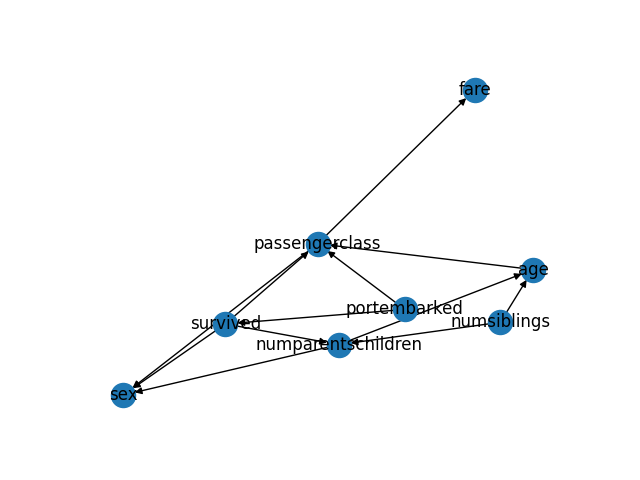
\includegraphics[width=0.6\textwidth]{small_path.png}
    \caption{Path with largest Bayes score for the `Small' dataset}
\end{figure}

\begin{figure}[h]
    \centering
    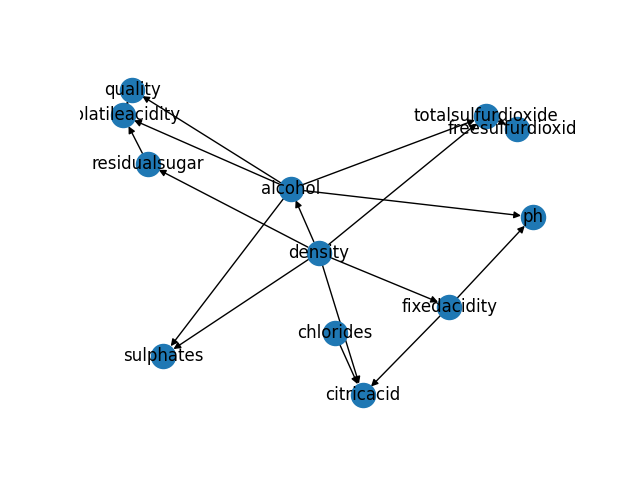
\includegraphics[width=0.6\textwidth]{medium_path.png}
    \caption{Path with largest Bayes score for the `Medium' dataset}
\end{figure}

\begin{figure}[h]
    \centering
    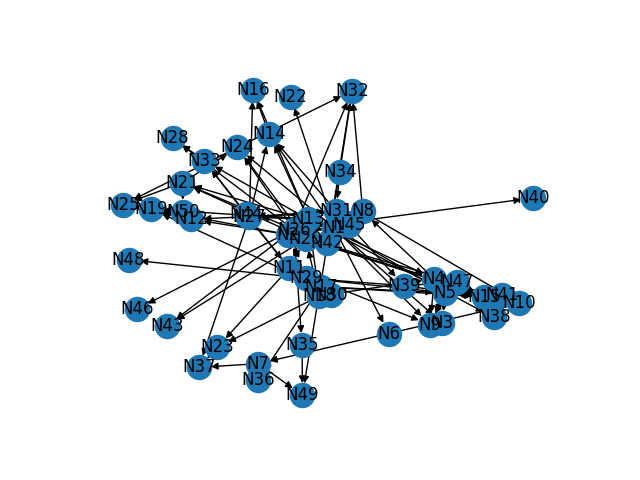
\includegraphics[width=0.6\textwidth]{large_path.png}
    \caption{Path with largest Bayes score for the `Large' dataset}
\end{figure}

%===========================================



\section{Code}
%===========================================
%===========================================
The first code block  implements my search algorithm. I provide additional code blocks beneath this one, organized in separate sections with additional utility functions to support this code
\begin{algorithm}
\begin{small}
\begin{lstlisting}[language=Python]
import numpy as np
import pandas as pd
import networkx as nx
import matplotlib.pyplot as plt
import time

from k2_search import k2_search # see blocks below
from local_search import local_search # see blocks below


def read_data(filename):
    # read in data    
    raw_data = pd.read_csv(f'./data/{filename}.csv')
    df, nodes = raw_data.values, list(raw_data.columns)
    
    return nodes, df

def save_results(G, filename):
    # save graph image
    plt.plot(figsize=(15, 15))
    nx.draw(G, with_labels=True)
    plt.savefig(f'./writeup/results/{filename}_path.png')
    
    # save graph file
    with open(f'{filename}.gph', 'w') as f:
        for edge in G.edges():
            f.write(f'{edge[0]}, {edge[1]}\n')
    return

# graph search algorithm
def random_start_graphsearch(nodes, data, iterations=3):
    time_total = -time.time()
    time_mean_iter = 0
    bscore_best, G_best = -np.inf, np.nan
    
    for i in range(iterations):
        time_mean_iter -= time.time()
        
        # shuffle nodes
        rs_idx = np.random.choice(
            np.arange(len(nodes)), size=len(nodes), replace=False)
        rs_nodes = [nodes[r] for r in rs_idx]
        rs_data = data[:,rs_idx]
        
        # run k2 search
        G_cand, bscore_cand, __ = k2_search(
            rs_nodes, rs_data, max_par_nodes=None)
        # run local search
        G_cand, bscore_cand, __ = local_search(
            G_cand, rs_nodes, rs_data, max_iter=20)
        
        if bscore_cand > bscore_best:
            bscore_best = bscore_cand
            G_best = G_cand
        
        time_mean_iter += time.time()
        
    time_total += time.time()
    time_mean_iter /= iterations
    
    return G_best, bscore_best, (time_total, time_mean_iter)


def main():
    if len(sys.argv) != 3:
        raise Exception("usage: python project1.py <filename prefix> n_iterations")

    filename = sys.argv[1]
    n_iterations = int(sys.argv[2])
    results = {}

    # read data
    print('reading data...')
    nodes, df = read_data(filename)

    # get graph with best bayescore
    print('getting best graph...')
    G, bayescore, total_times = random_start_graphsearch(
        nodes, df, iterations=n_iterations, local=True)

    # save results
    print('saving results...')
    save_results(G, filename)

    # print table output
    results['Bayes score'] = [np.round(bayescore, 3)]
    results['Graph structure (N, E)'] = [f'({len(G.nodes)}, {len(G.edges)})']
    results['Total time (sec)'] = [np.round(total_times[0], 3)]
    results[f'Mean iteration time (sec, {n_iterations} iters)'] = [
        np.round(total_times[1])]
    print(pd.DataFrame(results).T.to_latex())
    
if __name__ == '__main__':
    main()

\end{lstlisting}
\end{small}
\end{algorithm}


\subsection{K2 search}
\begin{algorithm}
\begin{lstlisting}[language=Python]
import numpy as np
import networkx as nx
import scipy as sp
import time
import itertools

def get_M(G, data, nodes, query):
    parents = list(G.predecessors(query))
    
    # get all parent instances
    max_par_insts = np.zeros(len(parents)) 
    for i, pn in enumerate(parents):
        max_par_insts[i] = np.max(data[:,nodes.index(pn)])
    par_inst = np.array(list(
        itertools.product(*[np.arange(start=1, stop=mp+1) for mp in max_par_insts])), dtype=int)

    # make M matrix and alpha matrix
    max_query_inst = np.max(data[:, nodes.index(query)])
    M = np.zeros((len(par_inst), max_query_inst), dtype=int)
    alpha = np.ones_like(M)

    # for each parent instant find data rows that exist and populate M
    par_node_idx = [nodes.index(n) for n in parents]
    query_node_idx = nodes.index(query)
    for i, pi in enumerate(par_inst):
        # get rows in data with the parent instance
        d_idx = (data[:, par_node_idx] == pi).all(axis=1)
        # get query value for those rows
        query_vals = data[d_idx, query_node_idx]
        # increment query values
        for j in query_vals:
            M[i,j-1] += 1  
    
    return M, alpha

def get_bscore(G, data, nodes):
    score = 0
    for query in nodes:
        M, alpha = get_M(G, data, nodes, query)
        score += np.sum(sp.special.loggamma(M+alpha))
        score -= np.sum(sp.special.loggamma(alpha))
        score += np.sum(sp.special.loggamma(np.sum(alpha, axis=1)))
        score -= np.sum(sp.special.loggamma(np.sum(alpha, axis=1) + np.sum(M, axis=1)))
    
    return score

def k2_search(nodes, data, max_par_nodes=None):
    time_total = -time.time()
    
    if max_par_nodes is None:
        max_par_nodes = len(nodes)
        
    # initialize graph
    G = nx.DiGraph()
    G.add_nodes_from(nodes)
    bscore_best = get_bscore(G, data, nodes)
    
    # first node is oldest anscestor, loop through all potential children
    for i, chi_node in enumerate(nodes[1:]):
        bscore_cand, par_node_cand = -np.inf, np.nan
        par_node_count = 0

        # loop through all potential parents of a given child
        # add new edges that improve bscore until either 
        # max nodes are hit or there aren't any more parents
        while par_node_count < np.min((max_par_nodes, len(nodes[0:i+1]))):
            for par_node in nodes[0:i+1]:
                if not G.has_edge(par_node, chi_node):
                    G.add_edge(par_node, chi_node)
                    bscore_cand_trial = get_bscore(G, data, nodes)
                    if bscore_cand_trial > bscore_cand:
                        bscore_cand = bscore_cand_trial
                        par_node_cand = par_node
                    G.remove_edge(par_node, chi_node)

            # add the best parent
            if bscore_cand > bscore_best:
                bscore_best = bscore_cand
                par_node_count += 1
                G.add_edge(par_node_cand, chi_node)
            else: 
                break
    
    time_total += time.time()
                
    return G, bscore_best, time_total

\end{lstlisting}
\end{algorithm}


\subsection{Local search} 
\begin{algorithm}
\begin{lstlisting}[language=Python]
import numpy as np
import networkx as nx
import time

from k2_search import get_bscore

def move_to_rand_neighbor(G):
    n = len(G.nodes)
    i, j = np.random.choice(G.nodes(), size=2, replace=False)
    G_new = G.copy()
    
    # remove edge if there is one
    if G_new.has_edge(i, j):
        G_new.remove_edge(i, j)
        # with probability 0.5, add edge in opposite direction
        if np.random.random() > 0.5:
            G_new.add_edge(j, i)       
    # add edge if there is not one
    else:
        G_new.add_edge(i, j)
    return G_new

def is_cyclic(G):
    n_cycles = len(sorted(nx.simple_cycles(G)))
    return n_cycles != 0

def local_search(G, nodes, data, max_iter=25):
    time_total = -time.time()
    bscore_best = get_bscore(G, data, nodes)
    iters = 0
    
    while iters < max_iter:
        G_new = move_to_rand_neighbor(G)
        
        if is_cyclic(G_new):
            bscore_cand = -np.inf
        else:
            bscore_cand = get_bscore(G_new, data, nodes)
            
        if bscore_cand > bscore_best:
            bscore_best = bscore_cand
            G = G_new
            iters = 0
        else:
            iters += 1
        
    time_total += time.time()
            
    return G, bscore_best, time_total
    
\end{lstlisting}
\end{algorithm}

\end{document}